\documentclass{/home/janmebows/Documents/LatexTemplates/myassignment}
\title{Topic B Assignment 2}
\newcommand{\odd}[2]{\frac{d#1}{d#2}}

\begin{document}
\maketitle


\begin{enumerate}
	\item 
	\begin{enumerate}[label=(\roman*)]
		\item Let $S(t)$, $I(t)$ and $R(t)$ be the number of susceptible, infected and recovered people respectively at time $t$. We are modelling the SIR model where recovered individuals will die with rate $\mu$, and are reborn as susceptible. This is simply a transition from $R\to S$ with rate $\mu$. This is effectively an SIRS model. Writing out the transition table:
		\begin{table}[h]
		\centering
		\label{tab::sirsnaive}
		 	\begin{tabular}{c|c|c}
		 		Event&Transition&Rate\\
		 		\hline 
		 		Infection & $(S,I,R)\to (S-1,I+1,R)$ & $\frac{\beta IS}{S+I+R-1}$\\
		 		Recovery & $(S,I,R) \to (S,I-1,R+1)$ & $\gamma I$\\ 
		 		Rebirth & $(S,I,R)\to (S+1,I,R-1)$& $\mu R$
		 	\end{tabular}
		\label{tab::sirs}
		 	\begin{tabular}{c|c|c}
		 		Event&Transition&Rate\\
		 		\hline 
		 		Infection & $(S,I)\to (S-1,I+1)$ & $\frac{\beta IS}{N-1}$\\
		 		Recovery & $I \to I-1$ & $\gamma I$\\ 
		 		Rebirth & $S\to S+1$& $\mu (N-I-S)$
		 	\end{tabular}
		 	\caption{Top: full SIRS model description. Bottom: a simplified description to the model}
		 \end{table} 
		 Table~\ref{tab::sirsnaive} shows a na\"ive approach to the problem. Since rebirth occurs instantly after a recovered individual dies, $N$ remains fixed. 
		\begin{table}[h]
		\centering
		 \end{table} 
		\item %Deterministic approximation to the dynamics
		Without randomness, this is the system (using proportions)
		\begin{align*}
			\frac{di}{dt} &= \beta is - \gamma i\\
			\frac{ds}{dt} &= -\beta is + \mu(1-i-s)
		\end{align*}
		Where $I = Ni$ and $S = Ns$.
		\item %Long term behaviour of the deterministic approximation
			The long term behaviour of the deterministic system relates to its equilibria. I will consider the population proportions ($i,s$) rather than numbers ($I,S$).
			First get the $i$ nullclines:
			\begin{align*}
				\odd it = 0=\beta is -\gamma i\\
				\implies i=0 \ or \ \beta s - \gamma =0\\
				s = \frac{\gamma}{\beta}
			\end{align*}
			And the $s$ nullclines:
			\begin{align*}
				\odd st = 0 &= -\beta is+ \mu(1-i-s)\\
				-\beta is - \mu S &= -\mu(1-i)\\
				s(\beta i + \mu) &= \mu(1-i)\\
				s &= \frac{\mu(1-i)}{\beta i + \mu}
			\end{align*}
			So fixed points are: the trivial case: $i=0, s=1$, and the more interesting one:
			\begin{align*}
				s = \frac{\gamma}{\beta}, \quad \odd it &= -\beta i\frac{\gamma}{\beta} + \mu(1-i-\frac{\gamma}{\beta})\\
				0 &=-\gamma i + \mu  - \mu i - \mu\frac{\gamma}{\beta}\\
				\gamma i + \mu i &= \mu(1 - \frac{\gamma}{\beta})\\
				i &= \frac{\mu\left(1 - \frac{\gamma}{\beta}\right)}{\gamma + \mu}
			\end{align*}
			
			The fixed point for $I$ exists in the relevant region only if
			\begin{align*}
				1 - \frac{\gamma}{\beta} \geq0\\
				\gamma \leq \beta
			\end{align*}
			So this fixed point exists only if $\gamma \leq \beta$

			The stability of these steady states, using the Jacobian:
			\[J(i,s) = \begin{pmatrix}
				\beta s - \gamma & \beta i\\
				-\beta s - \mu &-\beta i - \mu
			\end{pmatrix}\]
			And hence for the steady states
			\[J(0,1) = \begin{pmatrix}
				\beta - \gamma & 0\\
				-\beta - \mu & -\mu
			\end{pmatrix}\]
			With eigenvalues $\beta- \gamma$ and $-\mu$. This is stable if $\gamma > \beta$ and $\mu > 0$. If it is stable, in the long term it is an absorbing state. I.e. if $\gamma > \beta$ the system will eventually reach $(i,s) = (0,1)$ and remain there.

			For the other steady state:

			\begin{align*}
				J\left(\frac{\mu\left(1 - \frac{\gamma}{\beta}\right)}{\gamma + \mu},\frac\gamma\beta \right) &= \begin{pmatrix}
				\beta \frac\gamma\beta - \gamma & \beta \frac{\mu\left(1 - \frac{\gamma}{\beta}\right)}{\gamma + \mu}\\
				-\beta \frac\gamma\beta - \mu &-\beta \frac{\mu\left(1 - \frac{\gamma}{\beta}\right)}{\gamma + \mu} - \mu
			\end{pmatrix} \\
			&= \begin{pmatrix}
				0 & \frac{\mu(\beta - \gamma)}{\gamma + \mu}\\
				-\gamma - \mu & -\left(\frac{\mu(\beta - \gamma)}{\gamma + \mu} +\mu\right)
			\end{pmatrix}\\
			&= \begin{pmatrix}
					0 & \frac{\mu(\beta - \gamma)}{(\gamma + \mu)}\\
				-(\gamma + \mu) & -\frac{\mu(\beta - \mu)}{(\gamma + \mu)}
			\end{pmatrix}\\
			\end{align*}
			This will be stable if $\det J > 0 $ and $tr J <0$
			\begin{align*}
				\det J = \mu(\beta - \gamma) > 0\\
					\beta - \gamma > 0\\
					\beta > \gamma
			\end{align*}
			And the trace has to be negative:
			\begin{align*}
				-\mu(\beta - \mu) < 0\\
				\beta - \mu > 0\\
				\beta > \mu
			\end{align*}
			Hence this is a stable point so long as $\beta > \max\{\gamma,\mu\} $. I.e. in the long term we expect if this condition is true, the system will absorb into this equilibrium.


			If we have $\mu >\beta > \gamma > 0$ then there are no stable fixed points.

		\item %Simulate the stochastic model and compare long term dynamics to the deterministic
				%Consider R_0 = 15, 1/\gamma = 13 days, 1/\mu = 60 years 
				%and frequency dependent mixing
			The code to simulate the model is shown in Code~\ref{code:main}. Figure~\ref{fig:sirsim} plots 10 simulations of the model. Clearly for this parameter set, the number of infected goes to $0$. What is not shown in the plot is that as time goes to infinity $S\to N$.
		
			\begin{figure}[h]
				\centering
				\label{fig:sirsim}
				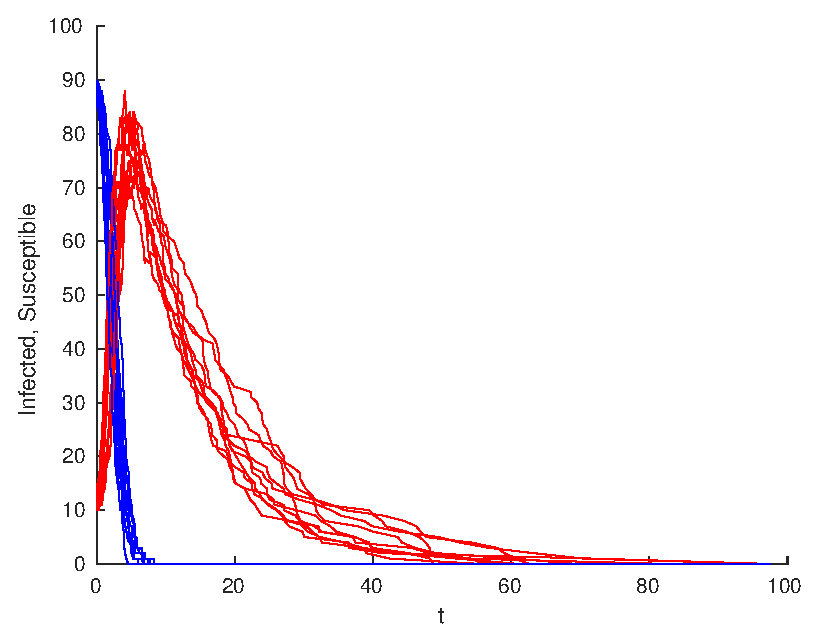
\includegraphics[width=\linewidth]{TopicBA2Q14}
				\caption{10 Simulations of the model for $R_0 =15$, $1/\gamma = 13$ and $1/\mu = \frac{60}{365}$. Blue: susceptible, red: infected}
			\end{figure}

		\item %Calculate E(I(t)) conditioned on the disease not going extinct and compare with the deterministic model
		%\[\mathbb{E}\left(I(t) | I(t) > 0\right)\]
		By simulating repeatedly, and rejecting points where $I(t)=0$ for any $t$, we can estimate $\mathbb{E}(I(t)|I(t) > 0)$. This is done in code~\ref{code:main} commented question 1 part 5

		Figure~\ref{fig:detandstoc} plots a comparison of the two models. Only $I(t)$ has been plotted for the deterministic and stochastic models, as this is the more interesting quantity. As shown in the figure, the two plots are very similar, overlapping for most of the region, but begin to separate slightly around $t=60$ and above.

		\begin{figure}[h]
			\centering
			\label{fig:detandstoc}
			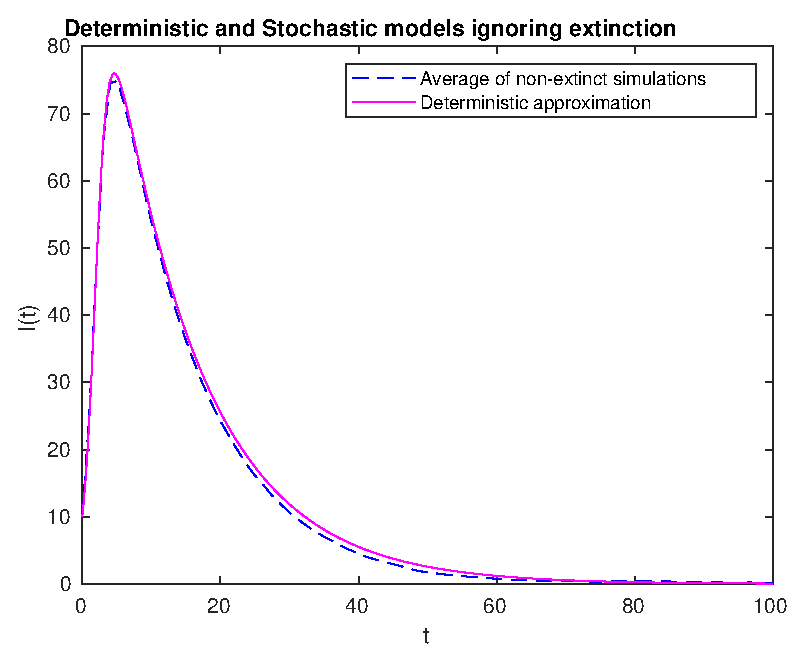
\includegraphics[width=\linewidth]{TopicBA2Q15}
			\caption{Comparison of the deterministic and stochastic models, where the stochastic solution is the average of 50 simulations.}
		\end{figure}


		\item %How would the model change if all individuals can die at a rate $\mu$ and 
				%susceptibles are born independently at rate $\mu$ proportional to the total population?
				If \textbf{all} individuals die at a rate $\mu$, and susceptible people are independently born at rate $\mu$ proportional to the total population, the model itself changes significantly. The total population size $N$ is no longer constant. The deterministic system of ODEs to model this is:
		\begin{align*}
			\frac{dI}{dt} &= \frac{\beta IS}{S+I+R} - \gamma I - \mu I\\
			\frac{dS}{dt} &= -\frac{\beta IS}{S+I+R} + \mu(I+R)\\
			\frac{dR}{dt} &= \gamma I -\mu R
		\end{align*}


	\end{enumerate}
	\item 
	\begin{enumerate}[label=(\roman*)]
		\item %Write code to generate the complete Q matrix for an SIR model (pop size N) using 
				%degree of advancement representation
				The code for this is shown in ~\ref{code:Qmat}. It calls code~\ref{code:DAmap} to obtain the DA representation and then generates a $Q_1$ and $Q_2$ matrix for infection and recovery rates, respectively.

		\item %For N=15, beta = 1.6, gamma =1 with IC (S(0),I(0)) = (N-1,1), produce
				%figures which show the PMF of I(t) at times 0,1,5,50. 
				%Use an implicit Euler method to numerically solve the forward equation
				Part 2 of code~\ref{code:main} utilises the SIRQ function and the code~\ref{code:IEMethodReturnAll}. Figure~\ref{fig:pmfI} displays bar-charts of the probability mass for number of people infected. Clearly at $t=0$ we expect no change to have occurred from the initial state. At $t=1$, there is a quite high probability $(\approx 0.43)$ that the disease has already died out, while the rest of the probability is decreasing as the number of infected increases. At $t=50$, with probability very close to $1$ there will be $0$ infected. 

				\begin{figure}[h]
					\centering
					\label{fig:pmfI}
					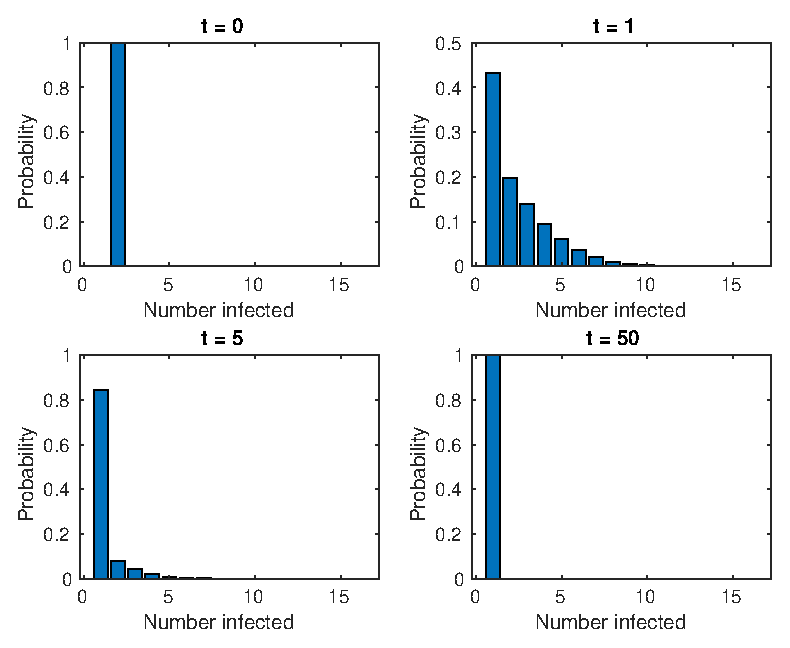
\includegraphics[width = \linewidth]{TopicBA2Q22.eps}
					\caption{Probability mass function of $I(t)$ calculated using the implicit Euler method for various times}
				\end{figure}
		\item %probability that exactly 12 people are infected over the course of the epidemic
				%same params as (ii)
				The code~\ref{code:main} outputs the value corresponding to $P\left(Z_1(end) = 12\right)$, i.e. the probability that exactly 12 people are infected over the epidemic, which is approximately $0.0501$. 

		\item %N=100,beta =1.6, gamma =1, plot the expected value of I(t) 
				%as a function of time by solving the forward equation numerically
				%and compare to the deterministic approximation from lectures
				The part labelled `Question 4 Part 4' of code~\ref{code:main} obtains the expected value of $I(t)$ via implicit Euler approximation and deterministic value. Figure~\ref{fig:detandstocEIT} shows the comparison between the deterministic value and implicit Euler approximation. The stochastic value (implicit Euler) will have much lower values for the expectation after $t=0$, since the probability of extinction at each step is quite high, whereas the deterministic model effectively ignores this.

		\begin{figure}[h]
			\centering
			\label{fig:detandstocEIT}
			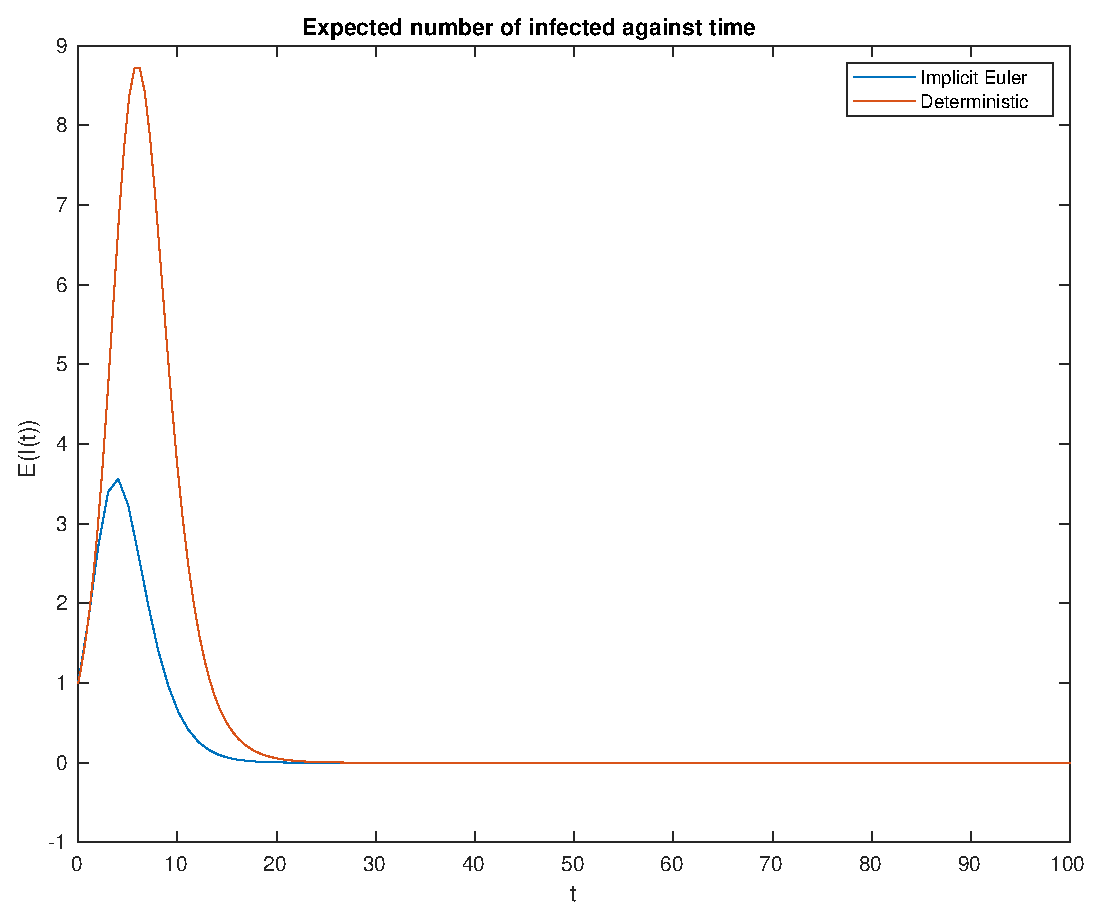
\includegraphics[width=\linewidth]{TopicBA2Q24}
			\caption{Comparison of the deterministic value and Implicit Euler approximation of $E[I(t)]$ .}
		\end{figure}
		\item %N=50,100,500 beta = 1.6 and gamma =1, calculate
				%probability of a minor outbreak using same methods as 3
				%How do these compare to the results derived using the branching process approx?

				The section `Question 2 part 5' of code~\ref{code:main} plots the expected total number of infections late into the infection.  
				
				It gives the plot figure~\ref{fig:probNumInfections}, and outputs the values:
				\begin{verbatim}

   (1,1)       0.7211
   (1,2)       0.7159
   (1,3)       0.6530

				\end{verbatim}
				These values are clearly decreasing. 
				\begin{figure}[h]
					\centering
					\label{fig:probNumInfections}
					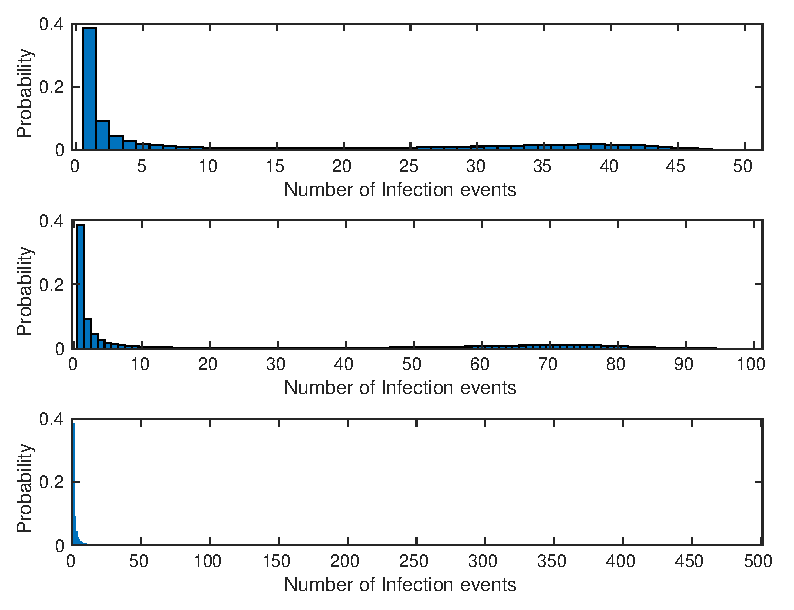
\includegraphics[width=\linewidth]{TopicBA2Q25}
					\caption{}
				\end{figure}

				From the branching process we found that the probability of a minor outbreak is:
				\[q = \min\{1,\gamma/\beta\}  = \frac{1}{1.6} = 0.625\]

				What we notice is that the values for $N\to \infty$ approach the value of $q = 0.625$
	\end{enumerate}
	\item 
	\begin{enumerate}[label=(\roman*)]
		\item %How do R0 and pmf of secondary infections change if we have 
				%erlang 2 dist infectious period with same mean 1/gamma 
				%instead of the normal exponential
				So we now consider the SI(2)R model. Transitions are
				\[S \stackrel{\frac{\beta IS}{N-1}}\to {I_1} \stackrel{\gamma}{\to} I_2 \stackrel{\gamma}{\to} R\]
				Since we are only considering a single individual in the system, the states correspond to those above. $R$ is the absorbing state.

				Since we consider an infinite population and we are only concerned with states that accumulate cost. So $Q_B$ will be the $Q$ matrix for $I_1,I_2$.
				\[Q_B = \begin{pmatrix}
					-2 \gamma& 2 \gamma\\
					0 & -2 \gamma\\
				\end{pmatrix}\]
				With cost function (since you infect at rate $\beta$ in either state):
				\[\vec f = \begin{bmatrix}
					\beta\\ \beta
				\end{bmatrix}\]
				Hence
				\begin{align*}
					Q_B \vec d = -\vec f\\
					\begin{pmatrix}
					-2 \gamma& 2 \gamma\\
					0 & -2 \gamma\\
					\end{pmatrix} \begin{bmatrix}
						d_1\\d_2
					\end{bmatrix} = \begin{bmatrix}
					-\beta\\ -\beta
				\end{bmatrix}\\
				\implies d_2 = \frac{\beta}{2\gamma}\\
				-2 \gamma d_1 +\beta = -\beta\\
				d_1 = \frac{\beta}{\gamma}
				\end{align*}
				Since $d_i$ are the expected cost for state $i$. So the expected total cost for one individual will be
				\[d_1 + d_2 = \frac{3 \beta}{2 \gamma}\]
				$R_0$ will be the expected number of secondary infections, which corresponds to $d_1$, i.e.
				\[R_0 = \frac{\beta}{\gamma}\]

				To calculate the PMF find the Laplace parameter:
				\[(Q_b - lF)\mathbf{L} = -\mathbf{a}\]

				\[\left(\begin{pmatrix}
					-2 \gamma& 2 \gamma\\
					0 & -2 \gamma
				\end{pmatrix} - l \begin{pmatrix}
					\beta&0\\0&\beta
				\end{pmatrix}\right)\begin{pmatrix}
					L_1\\L_2
				\end{pmatrix} = \begin{pmatrix}
					0\\
					-2\gamma
				\end{pmatrix} \]
				\[\implies (-2\gamma - l\beta)L_2 = -2\gamma\]
				Hence $L_2 = \frac{2\gamma}{2\gamma + l\beta}$

				\begin{align*}
					(-2\gamma-l\beta) L_1 + 2\gamma L_2 = 0	\\
					- \frac{L_1}{L_2} + L_2 = 0\\
					L_1 = L_2^2 = \left(\frac{2\gamma}{2\gamma + l\beta}\right)^2
				\end{align*}
				Now we have to invert this. Using the table of laplace inversions, we get 
				\[f_D(d) = 4\frac{\gamma^2}{\beta^2} d e^{-\frac{2\gamma}{\beta}d} \]
				Since $N_s(\sim Poi(D))$
				\begin{align*}
					P(N_s = k) &= \int_0^\infty \frac{e^{-d}d^k}{k!} \frac{4\gamma^2}{\beta^2} de^{-2\frac{\gamma}{\beta}d} dd\\
					&= \frac{4\gamma^2}{\beta^2k!}\int_0^\infty d^{k+1} e^{-d(1+2\frac{\gamma}{\beta})} dd\\
				\end{align*}
				Using integration by parts, $u = d^{k+1}$, $v' = e^{-d(1+2\frac{\gamma}{\beta})}$:
				\begin{align*}
					\int_0^\infty udv &= [uv]_0^\infty - \int_0^\infty vdu\\
					\int_0^\infty d^{k+1} e^{-d(1+2\frac{\gamma}{\beta})} dd&= \left[d^{k+1} \int e^{-d(1+2\frac{\gamma}{\beta})}dd\right]_0^{\infty} -(k+1)\int_0^{\infty} d^{k} \int e^{-d(1+2\frac{\gamma}{\beta})}dd dd\\
					&=  0 + \frac{1}{(1+2\frac{\gamma}{\beta})}(k+1)\int_0^{\infty} d^{k} e^{-d(1+2\frac{\gamma}{\beta})}dd\\
				\end{align*}
				By repeating this process...
				\begin{align*}
					\int_0^\infty d^{k+1} e^{-d(1+2\frac{\gamma}{\beta})} dd &= \frac{1}{(1+2\frac{\gamma}{\beta})}(k+1)! \int_0^\infty e^{-d(1+2\frac{\gamma}{\beta})}dd \\
					&= (k+1)! \left(\frac{1}{1 + 2\frac{\gamma}{\beta}}\right)^{k+2}
				\end{align*}
				
				And hence the PMF is
				\begin{align*}
					P(N_s = k) &= \frac{4\gamma^2}{\beta^2k!}(k+1)! \left(\frac{1}{1 + 2\frac{\gamma}{\beta}}\right)^{k+2}\\
					 &= \frac{4\gamma^2 k}{\beta^2} \left(\frac{\beta}{\beta+2\gamma}\right)^{k+2} \\
					 &= \frac{4\gamma^2 \beta^k (k+1)}{(\beta+2\gamma)^{k+2}} \\
				\end{align*}
				For non-negative integer $k$.

				
				
	
		\item %SIR CTMC N=20 where people need care to recover
				%4 people
				SIR model.	 We want to calculate 
				\[D = \mathbb{E}\left(\int_0^\infty f(X(t)) dt\right)\]
			 							
			With $N=20, \beta = 0.6$ and $1/\gamma = 3$, and the cost per day to take care of $i$ infected individuals will be:
			\[f(i) = ai + b\lceil\frac{i}{4}\rceil = 2i + 5\lceil\frac{i}{4}\rceil,\quad f(0) =0  \]
			Where $i=0$ is an absorbing state
			Have to solve the system 
			\[\vec d = -\vec f \backslash Q_b\]
			Where $d_i$ is the expected cost for caring for individuals given the process starts in state $i$.
			Since this is the SIR model, the code uses the DA state space. To extract the number of infected from this, $I = Z_1 - Z_2$. Figure~\ref{fig:expectedCost} plots the initial number of infected against the expected cost, with the assumption that initially no person has recovered from the infection. Clearly the maximum occurs for $I(0) = 20$, which makes sense since in this case, all people in the system must be cared for.
			The expected cost will be $220$.

			\begin{figure}[h]
				\centering
				\label{fig:expectedCost}
				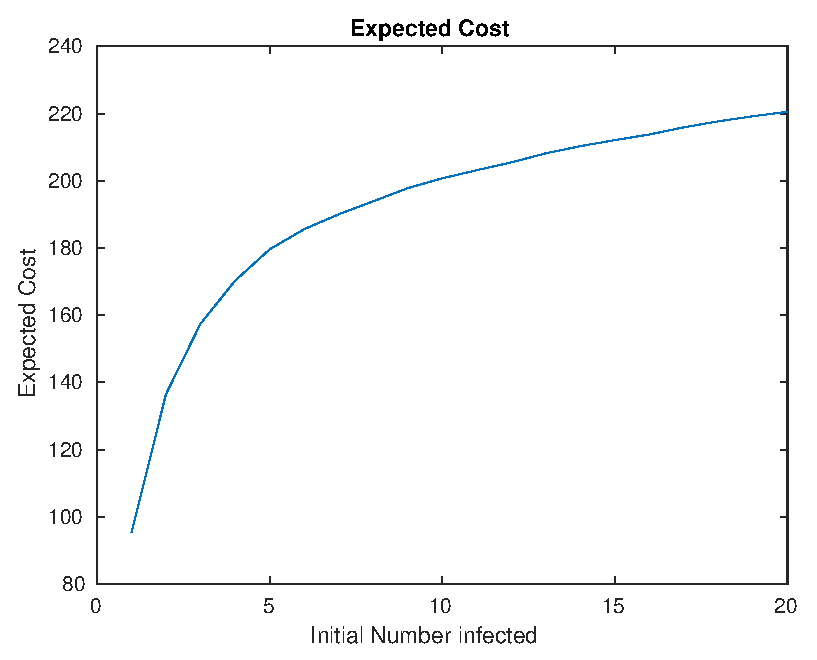
\includegraphics[width=\linewidth]{TopicBA2Q32}
				\caption{Expected cost given $i$ people were initially infected}
				
			\end{figure}
	\end{enumerate}
\end{enumerate}

\clearpage
\appendix
\section{Code}
\label{code:main}
\subsection{Main Script}
\lstinputlisting{DiseasesA2.m}

\label{code:SIRSsim}
\subsection{SIRS\_Sim.m}
\lstinputlisting{../SIRS_Sim.m}

\label{code:DAmap}
\subsection{SIR\_DA\_mapping.m}
\lstinputlisting{../SIR_DA_mapping.m}

\label{code:Qmat}
\subsection{SIRQ.m}
\lstinputlisting{../SIRQ.m}

\label{code:IEMethodReturnAll}
\subsection{IEMethodReturnAll.m}
\lstinputlisting{../IEMethodReturnAll.m}

\label{code:deterministic}
\subsection{SIRS\_DE\_deterministic.m}
\lstinputlisting{../SIRS_DE_deterministic.m}
	



\clearpage
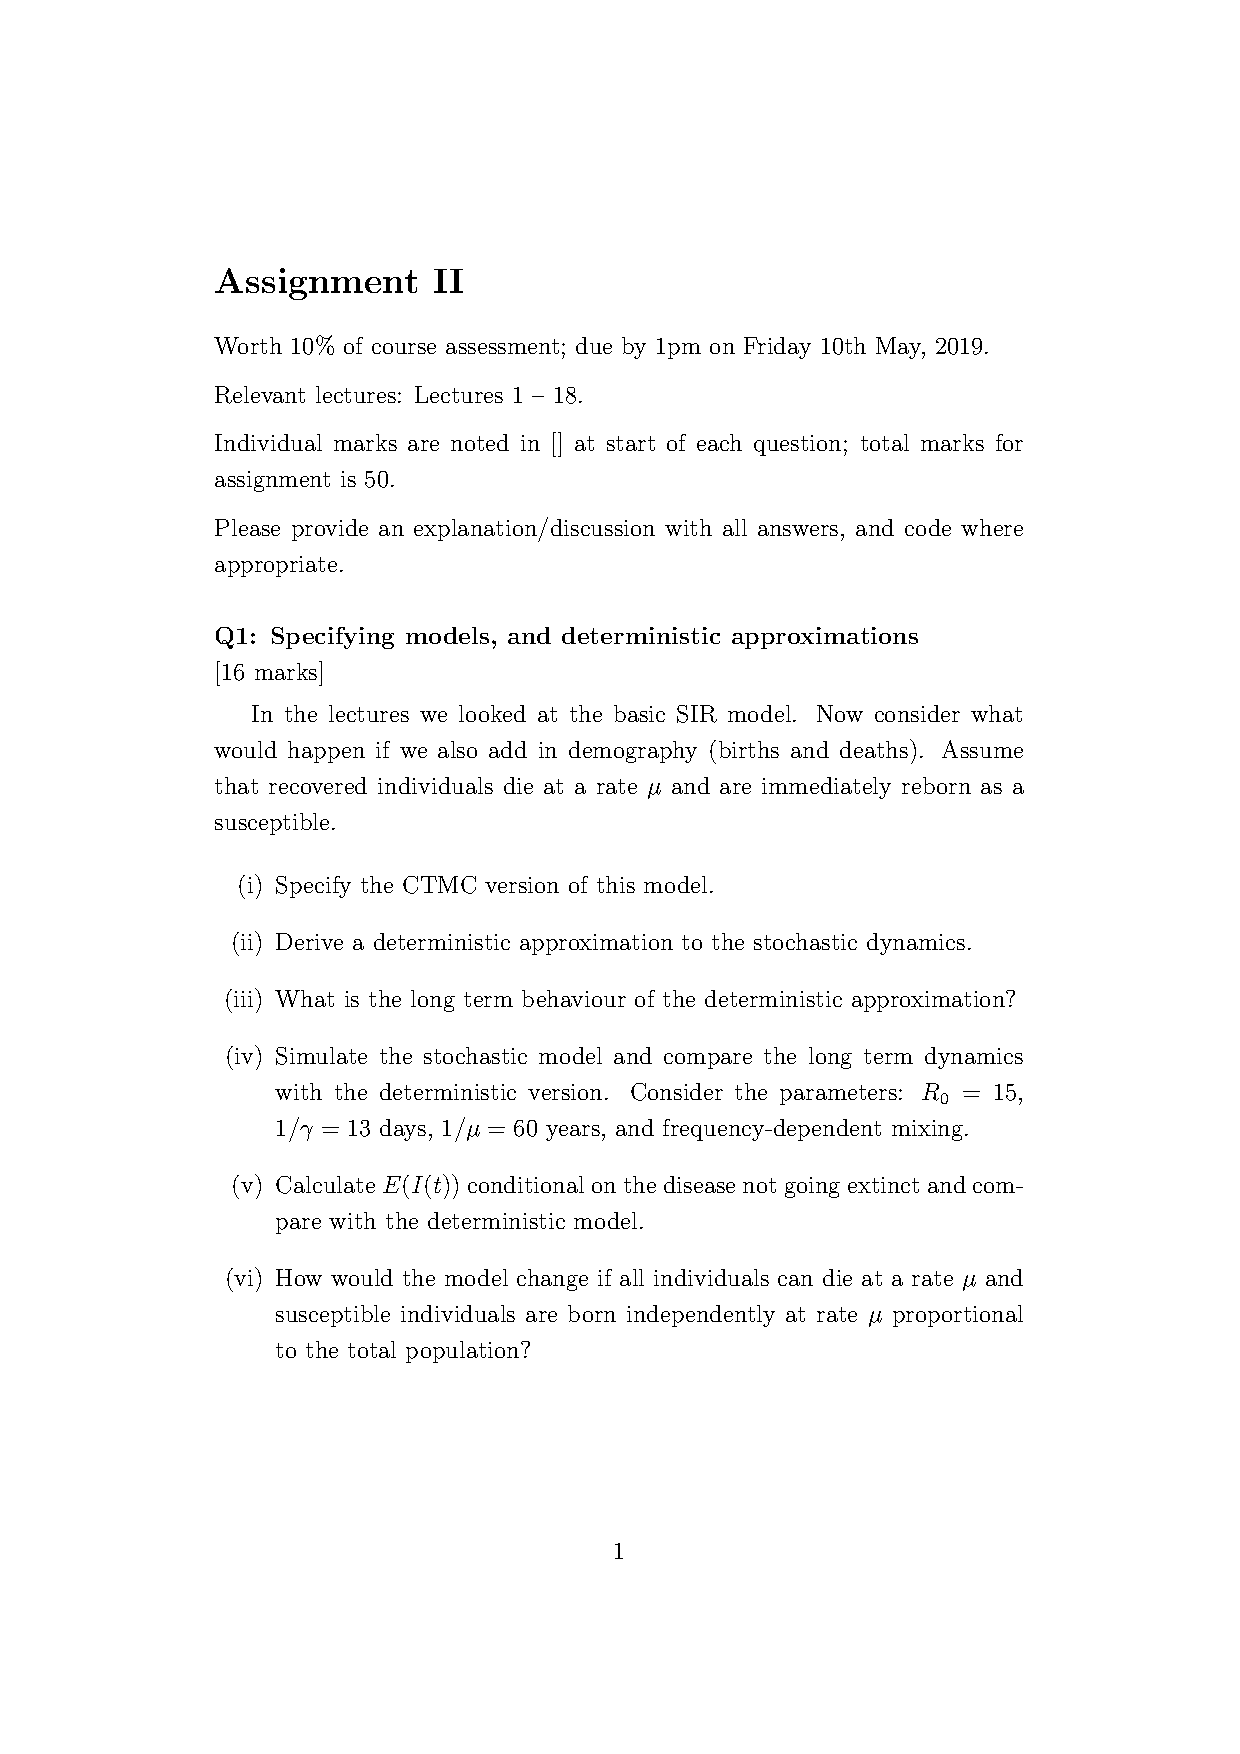
\includepdf[pages=1-]{TopicBA2Questions}
\end{document}